\documentclass[aspectratio=169]{beamer}
\usetheme[numbering=fraction]{metropolis}
\setbeamercolor{background canvas}{bg=white}  % true white, no border around figures

% --- NMBU accent color ---
\definecolor{nmbugreen}{HTML}{00705D}
\setbeamercolor{frametitle}{bg=nmbugreen}        % the top bar
\setbeamercolor{progress bar}{fg=nmbugreen}      % thin bar under title / on title page
\setbeamercolor{title separator}{fg=nmbugreen}   % rule on the title slide
\setbeamercolor{alerted text}{fg=nmbugreen}      % \alert{...}

\usepackage{appendixnumberbeamer}  % stop the frame total at \appendix
\usepackage{amsmath, amssymb, mathtools}
\usepackage{booktabs}        % \toprule etc. (thesis tables use these)
\usepackage{multirow}
\usepackage{subcaption}
\usepackage[style=numeric, sorting=none, giveninits=true, doi=true, maxbibnames=19, date=year, backend=biber]{biblatex}
\addbibresource{../bib.bib}
\setbeamertemplate{bibliography item}[text]   % show [1] labels instead of the article icon

% Figures: repo-root figures/ first, then thesis-local figures/
\graphicspath{{../../figures/}{../figures/}}

% --- Title metadata ---
\title{Efficient Low-Rank Methods for\\ PDE-Based Inverse Problems}
\subtitle{Forsvar av masteroppgave}
\author{Elias Jegervatn Severinsen}
\institute{
  Norges miljø- og biovitenskapelige universitet
  \\ Datavitenskap}
\date{2026 \\ \footnotesize Veiledere: Ole L. Elvetun, Jonas Kusch}

\begin{document}

\maketitle

\begin{frame}{Oversikt}
  \tableofcontents
\end{frame}

% =====================================================================
\section{Motivasjon: et PDE-basert inverst problem}
% =====================================================================

\begin{frame}{Det inverse problemet}
Betrakt problemet
\begin{equation*}
  \begin{aligned}
    -\nabla \cdot \sigma\nabla u + c u &= f \quad \text{i } \Omega, \\
    \tfrac{\partial u}{\partial n} &= 0 \quad \text{på } \partial\Omega.
  \end{aligned}
\end{equation*}
\begin{itemize}
  \item \textbf{Forover:} gitt $f$, finn $u$.
  \item \textbf{Inverst:} gitt rand-data $u|_{\partial\Omega}$, rekonstruer $f$.
\end{itemize}
\pause
Om vi definerer $\mathcal K = \mathcal T \circ \mathcal S$, med $\mathcal{T}: u \to u|_{\partial\Omega}$ og $\mathcal{S}: f \to u$, får vi formuleringen:
\begin{equation*}
  \mathcal K f = u|_{\partial\Omega}.
\end{equation*}
\end{frame}


\begin{frame}{Foroveroperatoren}
\centering
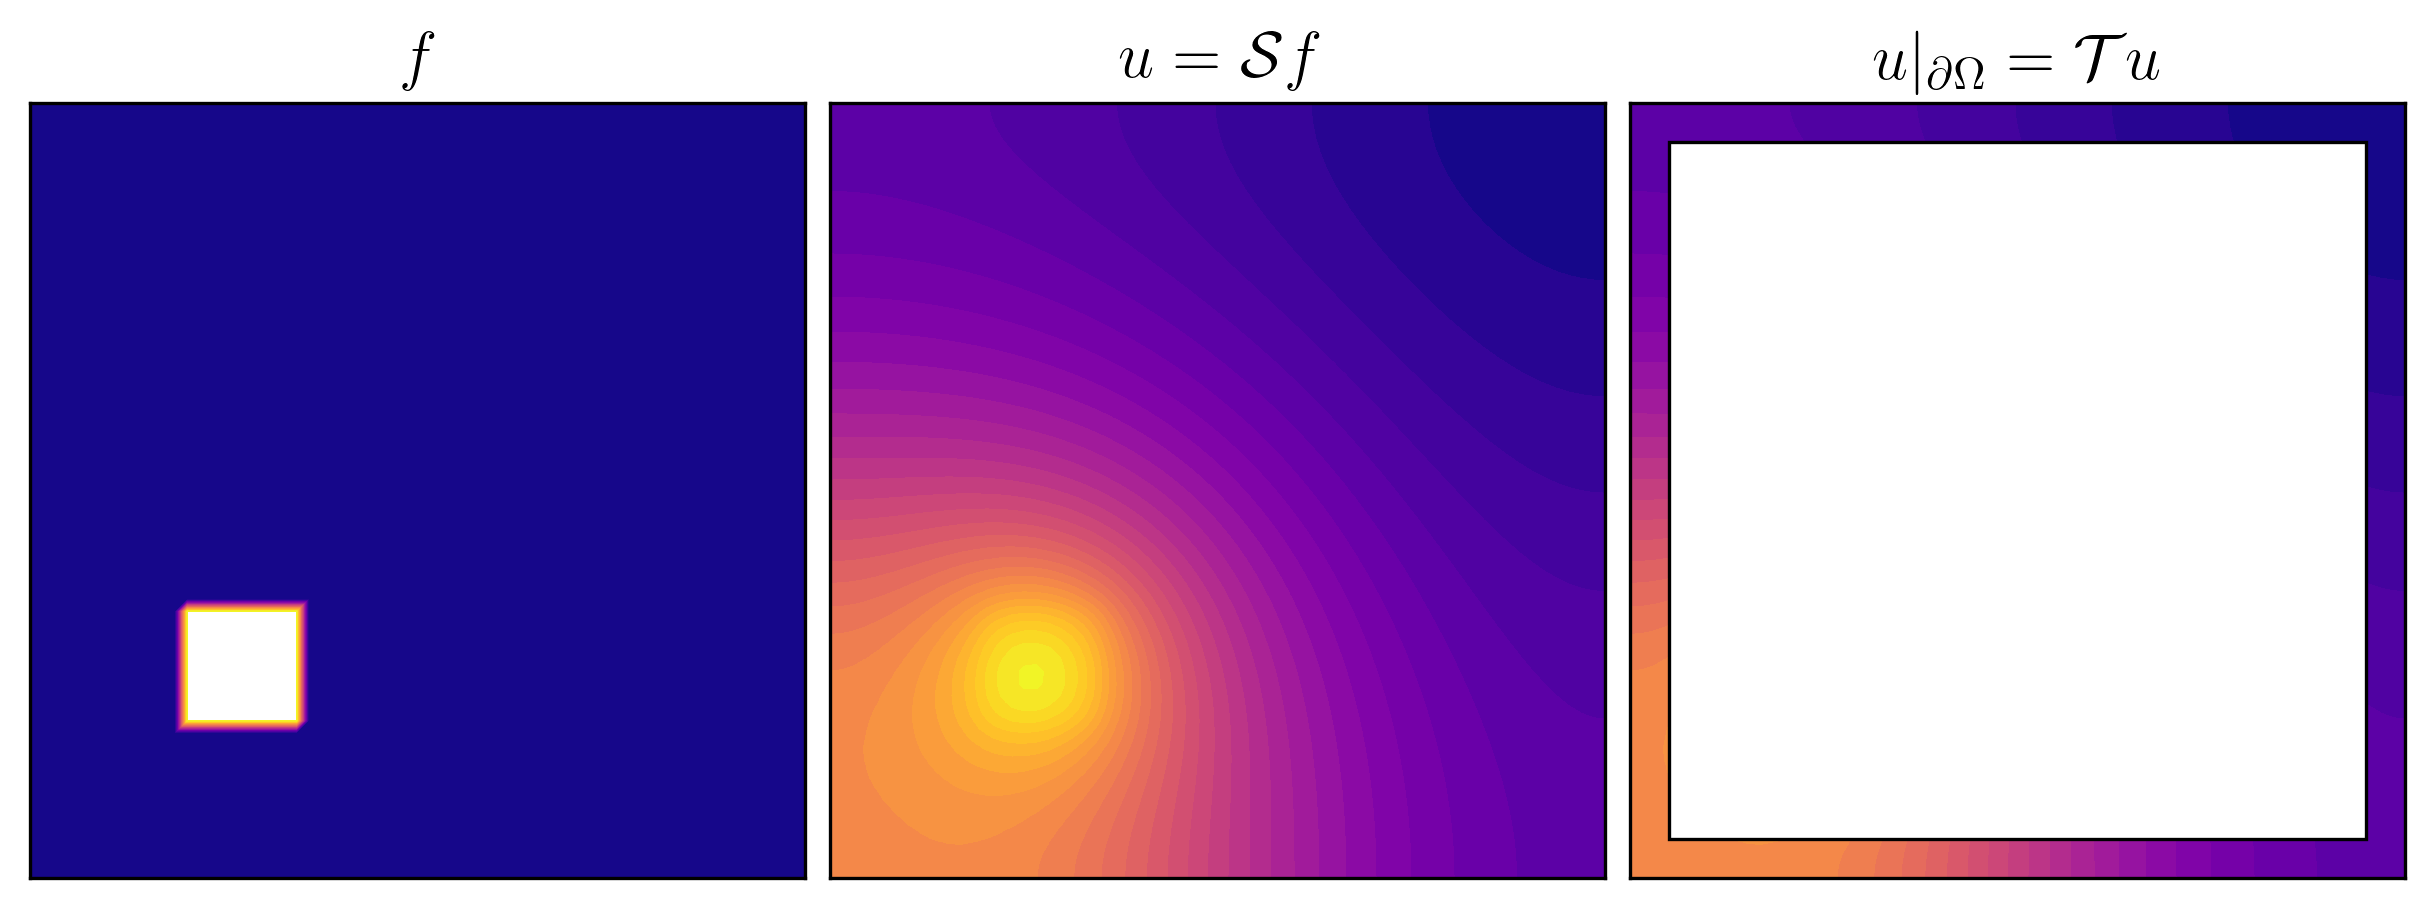
\includegraphics[width=0.85\linewidth]{forward_illustration}
\end{frame}


\begin{frame}{Utfordringen: $\mathcal{K}$ er dårlig stilt og forventningsskjev}
La $K \in \mathbb{R}^{N_b \times N}$ være diskretiseringen av $\mathcal{K}$, med $N$ noder og $N_b$ rand-noder
\begin{itemize}
  \item $K$ er svært dårlig stilt, siden...
  \item<2-> $K$ har et stort nullrom: løsningene er ikke-entydige
  \item<3-> $K$ har raskt avtagende singulærverdier: løsningene er ustabile
\end{itemize}
\onslide<4->{
Tikhonov-regularisering er en standard prosedyre,
\begin{equation*}
  \min \| K x - y \|_{M_\partial}^2 + \lambda^2 \| W x \|_M^2,
\end{equation*}
men dette gir forventningsskjeve løsninger som konsentrerer seg nær randen av domenet \cite{elvetunRegularizationOperatorSource2020}.
}
\end{frame}

% =====================================================================
\section{Tidligere arbeid: vektet Tikhonov-regularisering}
% =====================================================================

\begin{frame}{Elvetun og Nielsens vekter}
$f$ kan skrives som $f = f_\perp + f_0$. Elvetun og Nielsen viser at $f$ nær $\partial \Omega$ har større $f_\perp$-komponent:
\begin{itemize}
  \item<2-> La $\hat P: V_h \to \operatorname{Nul}(\mathcal{K})^\perp$
  \item<3-> Minimum-norm-løsningen $f^* = \sum_i \langle \hat P f,\, \phi_i \rangle \phi_i$
  \item<4-> $\| \hat P \phi_i \| = \| \phi_{i,\perp} \|$ blir liten for $\phi_i$ langt unna $\partial \Omega$
  \item<5-> Komponenten $\langle \hat P f,\, \phi_i \rangle$ tvinges til å bli liten fra Cauchy-Schwarz
\end{itemize}
\onslide<6->{
De retter opp i denne skjevheten ved å sette $\| \hat P \phi_i \| = 1$ for alle $i$:
\begin{equation*}
  w_i = \|K^+ K e_i \|,\quad W = \operatorname{diag}(w_1,\dots,w_N)
\end{equation*}
}
\end{frame}


\begin{frame}{Elvetun og Nielsens vekter: utfordringen}
Men denne prosedyren er beregningskrevende:
\begin{itemize}
  \item<2-> Å konstruere $K$ krever å løse $N_b$ lineære systemer: $\mathcal{O}(N_b N \log N)$
  \item<3-> Å finne $K^+$ krever en SVD, som koster $\mathcal{O}(N_b^2 N)$
  \item<4-> $N$ skalerer som $\mathcal{O}(n^2)$ i 2D, og $\mathcal{O}(n^3)$ i 3D: uegnet for store problemer
\end{itemize}
\end{frame}


% =====================================================================
\section{Tilnærming av foroveroperatoren: matrise-fri rSVD}
% =====================================================================

\begin{frame}{Tilnærming av foroveroperatoren}
$K$ har et stort nullrom ($\operatorname{rank}(K) = N_b$) og raskt avtagende singulærverdier:

\centering
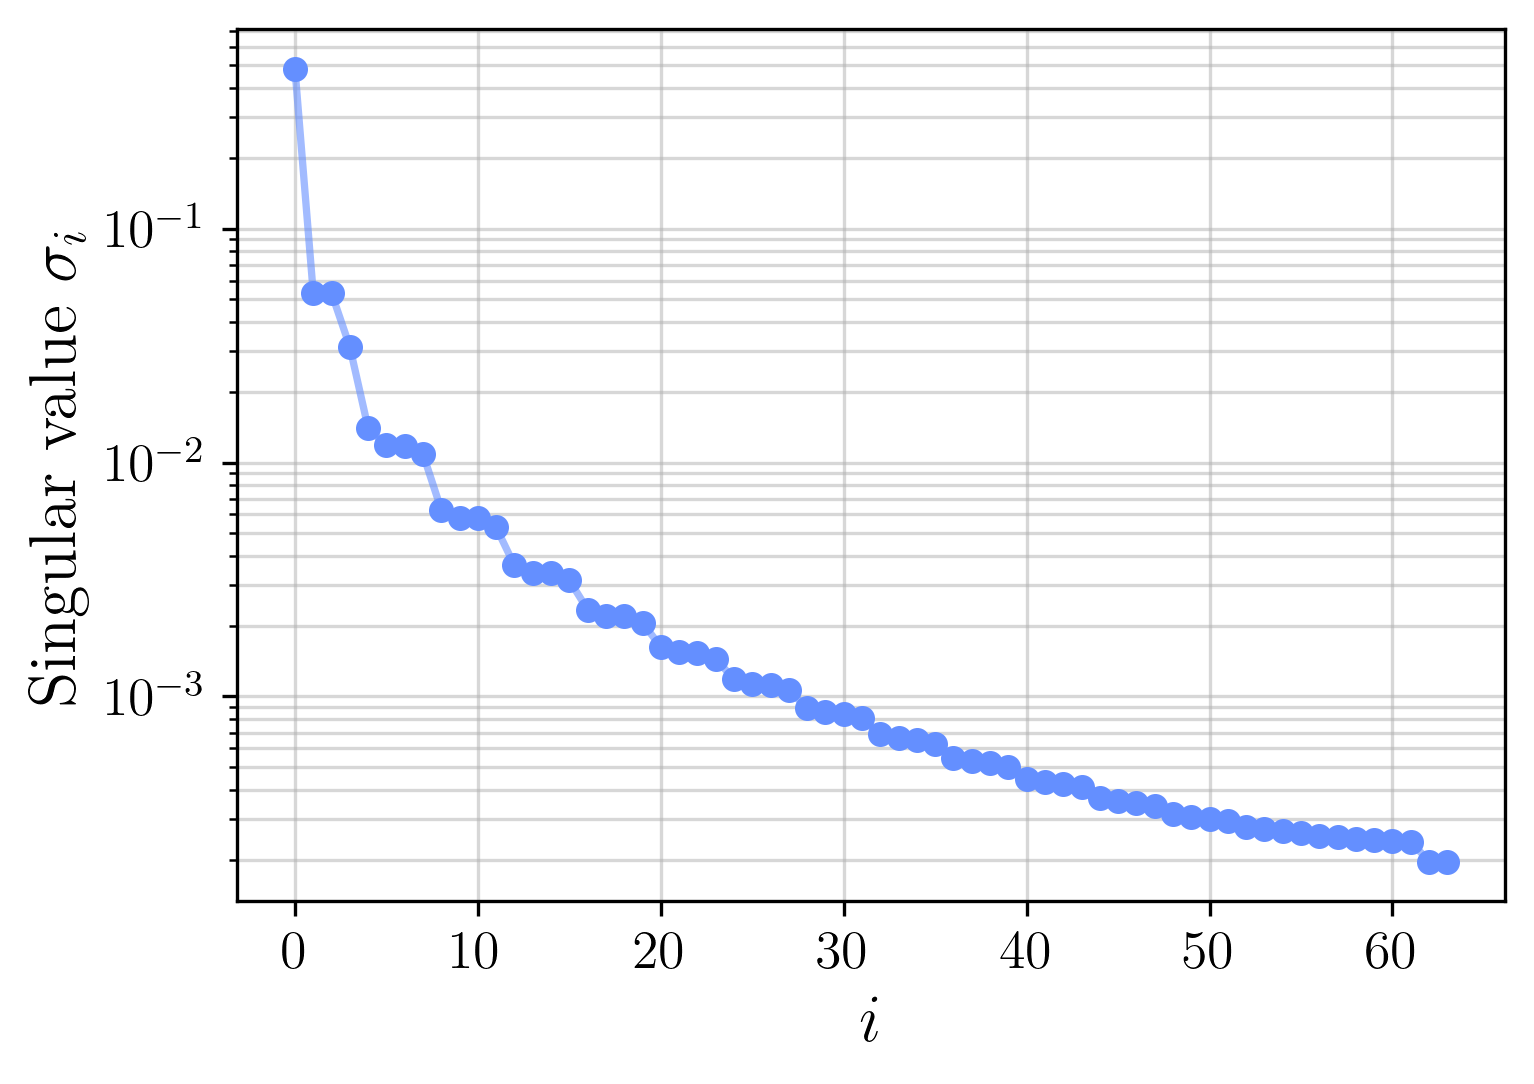
\includegraphics[width=0.4\linewidth]{singular_values.png}

\begin{itemize}
  \item<2-> En rang-$k$-tilnærming $K \approx U \Sigma V^T$ kan approksimere $K$ godt for små $k$
  \item<3-> \textbf{Idé:} bruk den randomiserte SVD-en (rSVD) til å finne $U \Sigma V^T$ \cite{halkoFindingStructureRandomness2011}
  \item<4-> Vektene tilnærmes via $w_i = \| K^+ K e_i \| \approx \| V V^T e_i \|$
\end{itemize}
\end{frame}

\begin{frame}{En matrise-fri rSVD}
Den klassiske rSVD-en finner $K \approx U \Sigma V^T$:
\begin{itemize}
  \item<2-> Sampling: $Y = K \Psi$
  \item<3-> Range-tilnærming: $QR = Y$
  \item<4-> SVD-tilnærming: $B = Q^T K$, $QQ^T K = QB = (Q \tilde U)\Sigma V^T = U \Sigma V^T$ 
\end{itemize}

\onslide<5->{
Hvordan finner vi $B = Q^T K$ om vi ikke har $K$?
\begin{itemize}
  \item<6-> Bruk identiteten $K = M_\partial^{-1} (K^*)^T M$
  \item<7-> Det gir $B = (K^* M_\partial^{-1} Q)^T M$
  \item<8-> Matrise-fri rSVD: $K \approx U \Sigma V^T$ ved å anvende $K$ og $K^*$ $l = k + p$ ganger
\end{itemize}  
}
\end{frame}

% =====================================================================
\section{Matrise-fri rSVD: resultater}
% =====================================================================

\begin{frame}{rSVD: beregningstid}
  \centering
  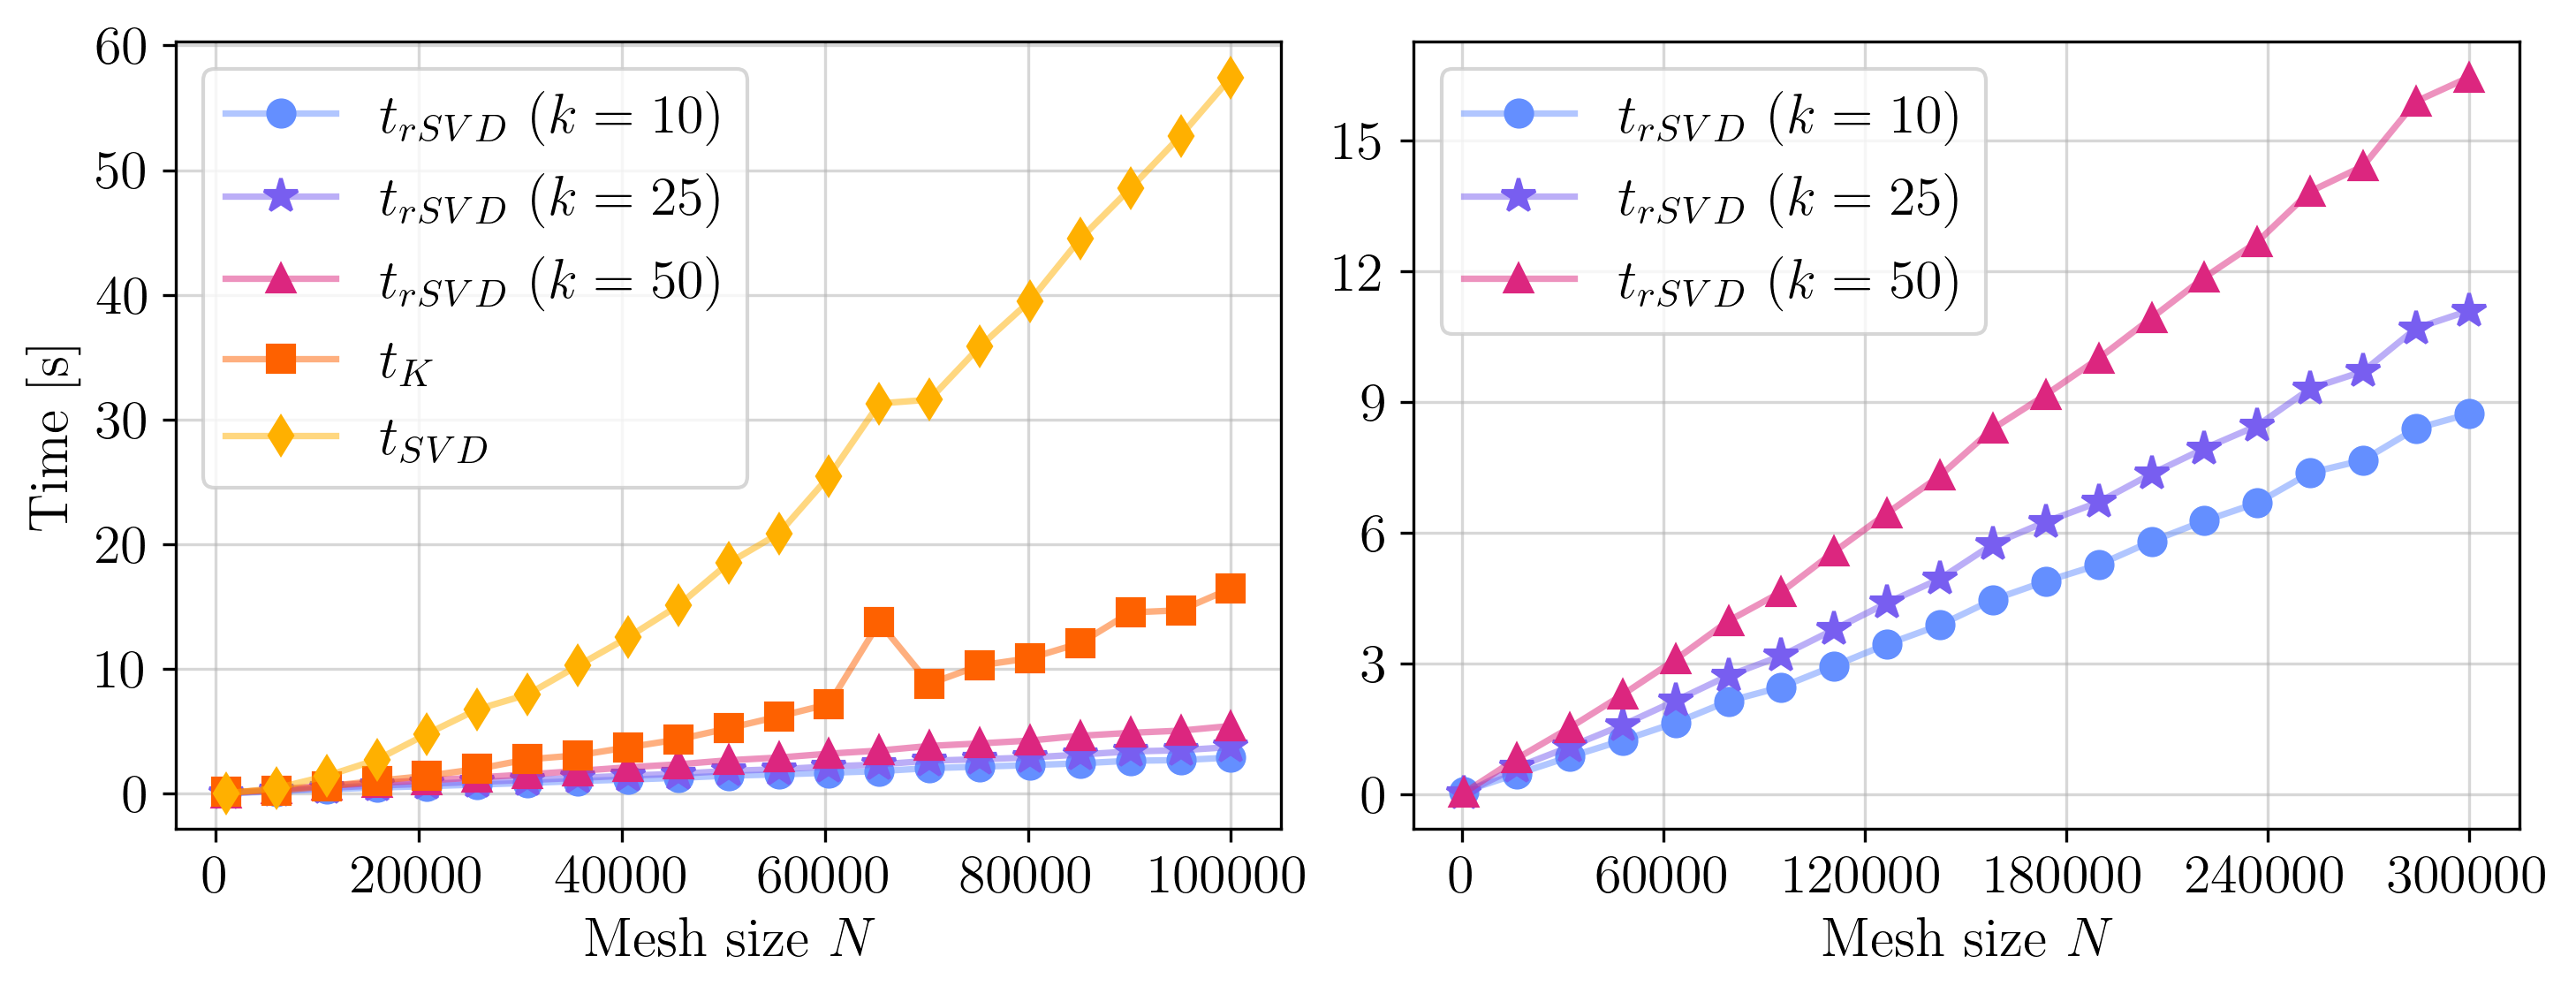
\includegraphics[width=0.8\linewidth]{rsvd_computational_time_comp.png}
  \par\medskip
  \footnotesize rSVD versus å danne $K$ eksplisitt ($t_K$) og å finne dens SVD ($t_{\text{SVD}}$).
\end{frame}


\begin{frame}{rSVD: vektede Tikhonov-løsninger}
\centering
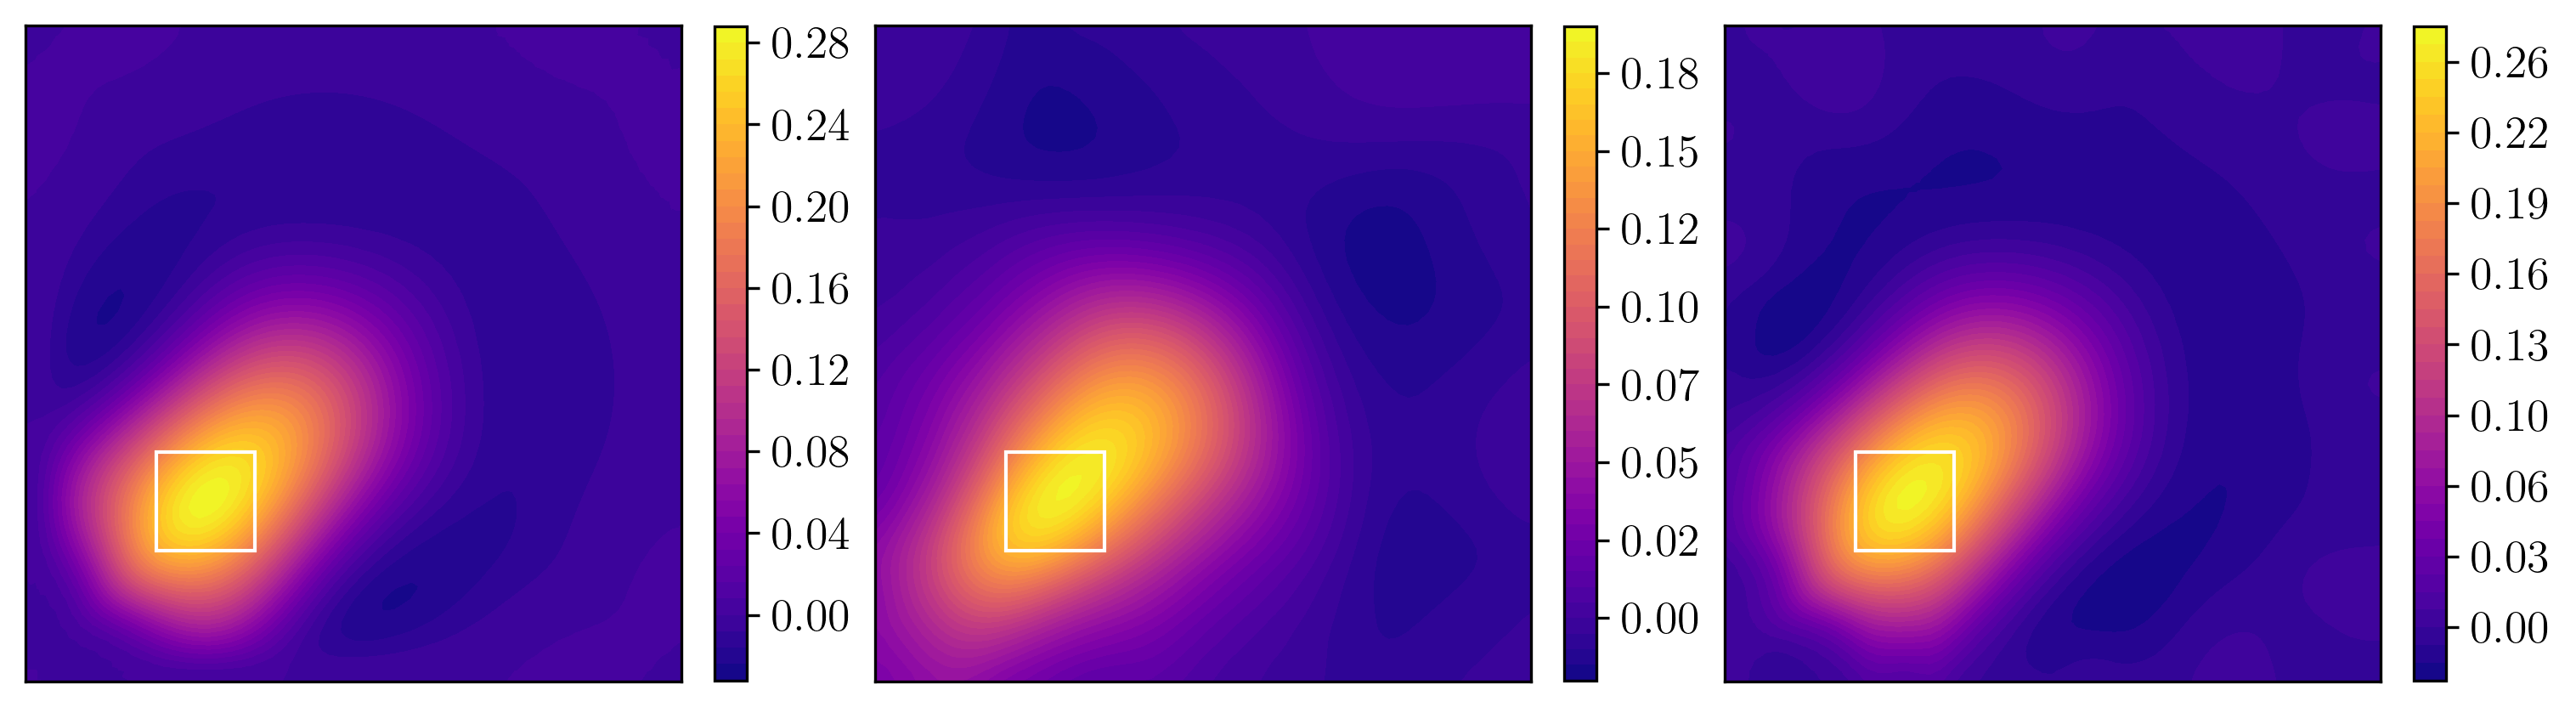
\includegraphics[width=0.8\linewidth]{test_problem_I.png}
\par\medskip
\footnotesize Vektede Tikhonov-løsninger med eksakt $K$ og $W$ (venstre), en rang-10-rSVD-tilnærming av $K$ og $W$ (midten), og en rang-50-rSVD-tilnærming (høyre).
\end{frame}


\begin{frame}{rSVD: evalueringsmetrikker}
Vi målte feilen ved bruk av
\begin{itemize}
  \item<2-> Euklidisk norm: måler elementvis amplitude
  \item<3-> Earth mover’s distance (EMD): måler forskjell i ``massene''
  \item<4-> AUC-IoU: måler overlapp
\end{itemize}
\onslide<5->{
\centering
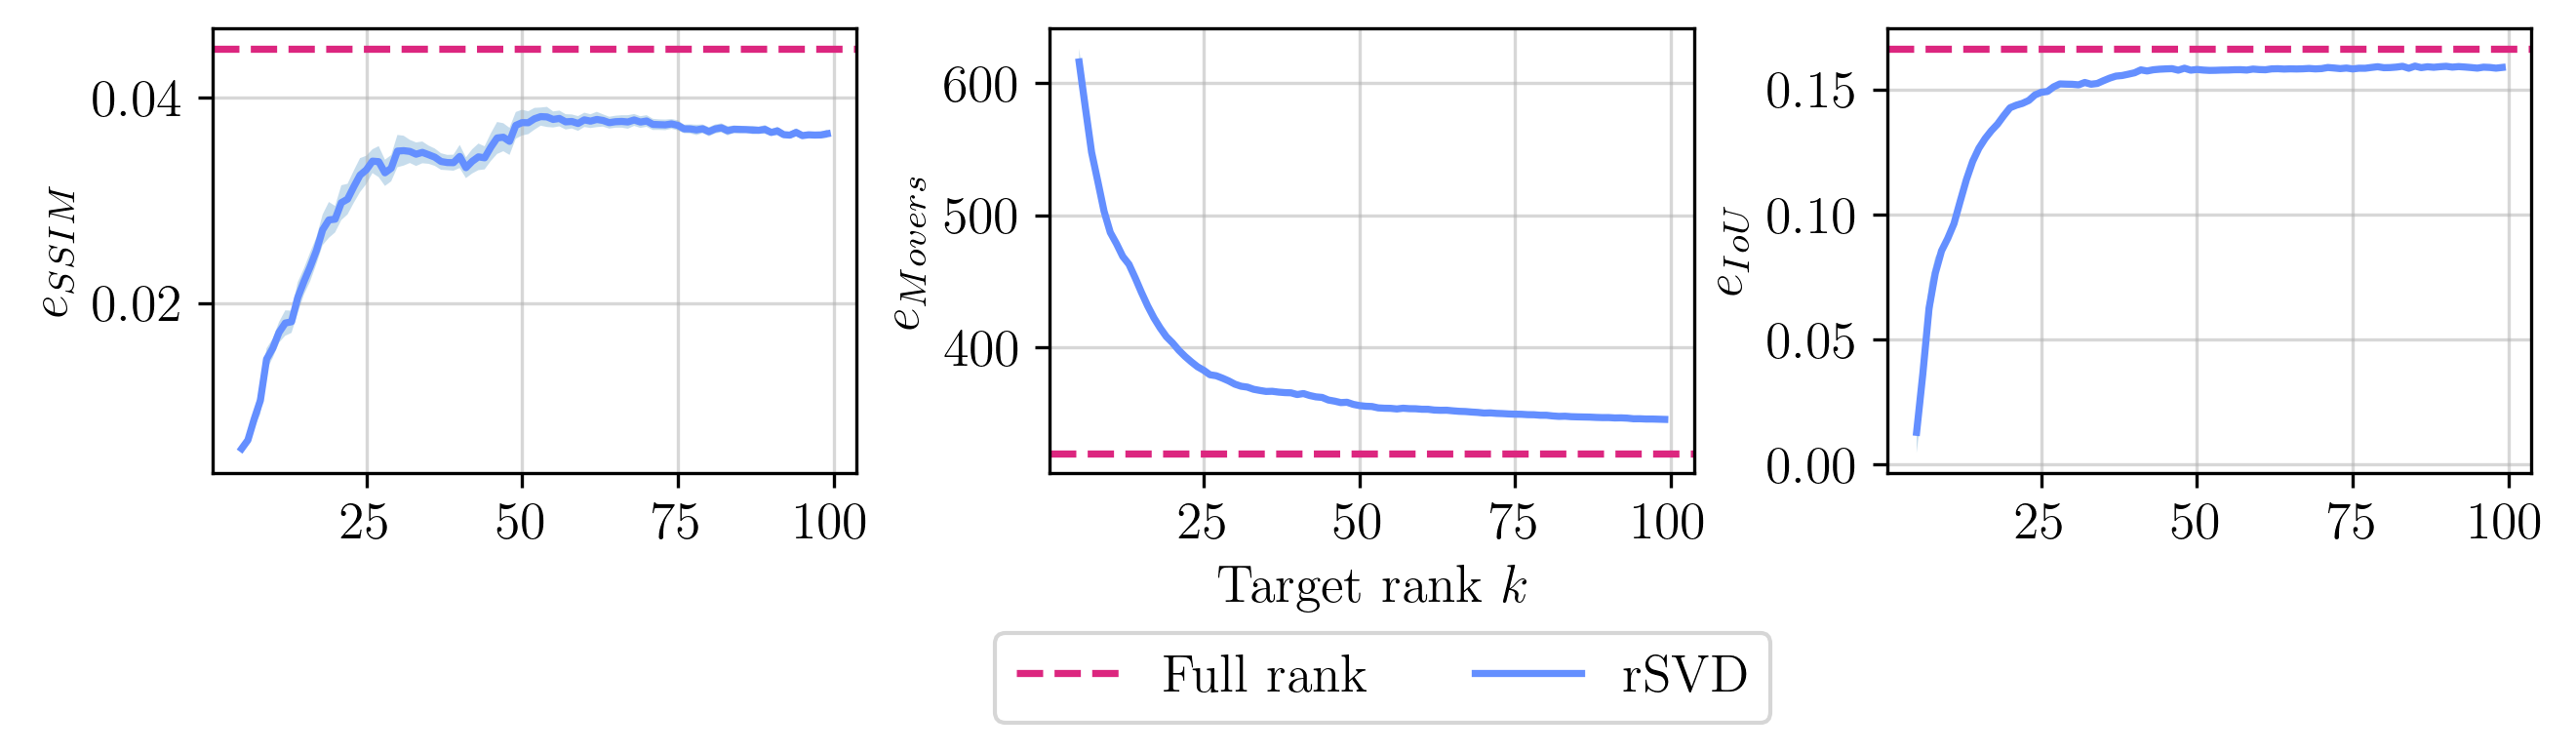
\includegraphics[width=0.8\linewidth]{rsvd_over_k_I.png}
\par\medskip
\footnotesize Euklidisk norm (venstre), EMD (midten), og AUC-IoU (høyre).
}
\end{frame}

% =====================================================================
\section{Dynamisk lavrang-tilnærming (DLRA)}
% =====================================================================

\begin{frame}{Lavrang-løsninger}
\begin{center}
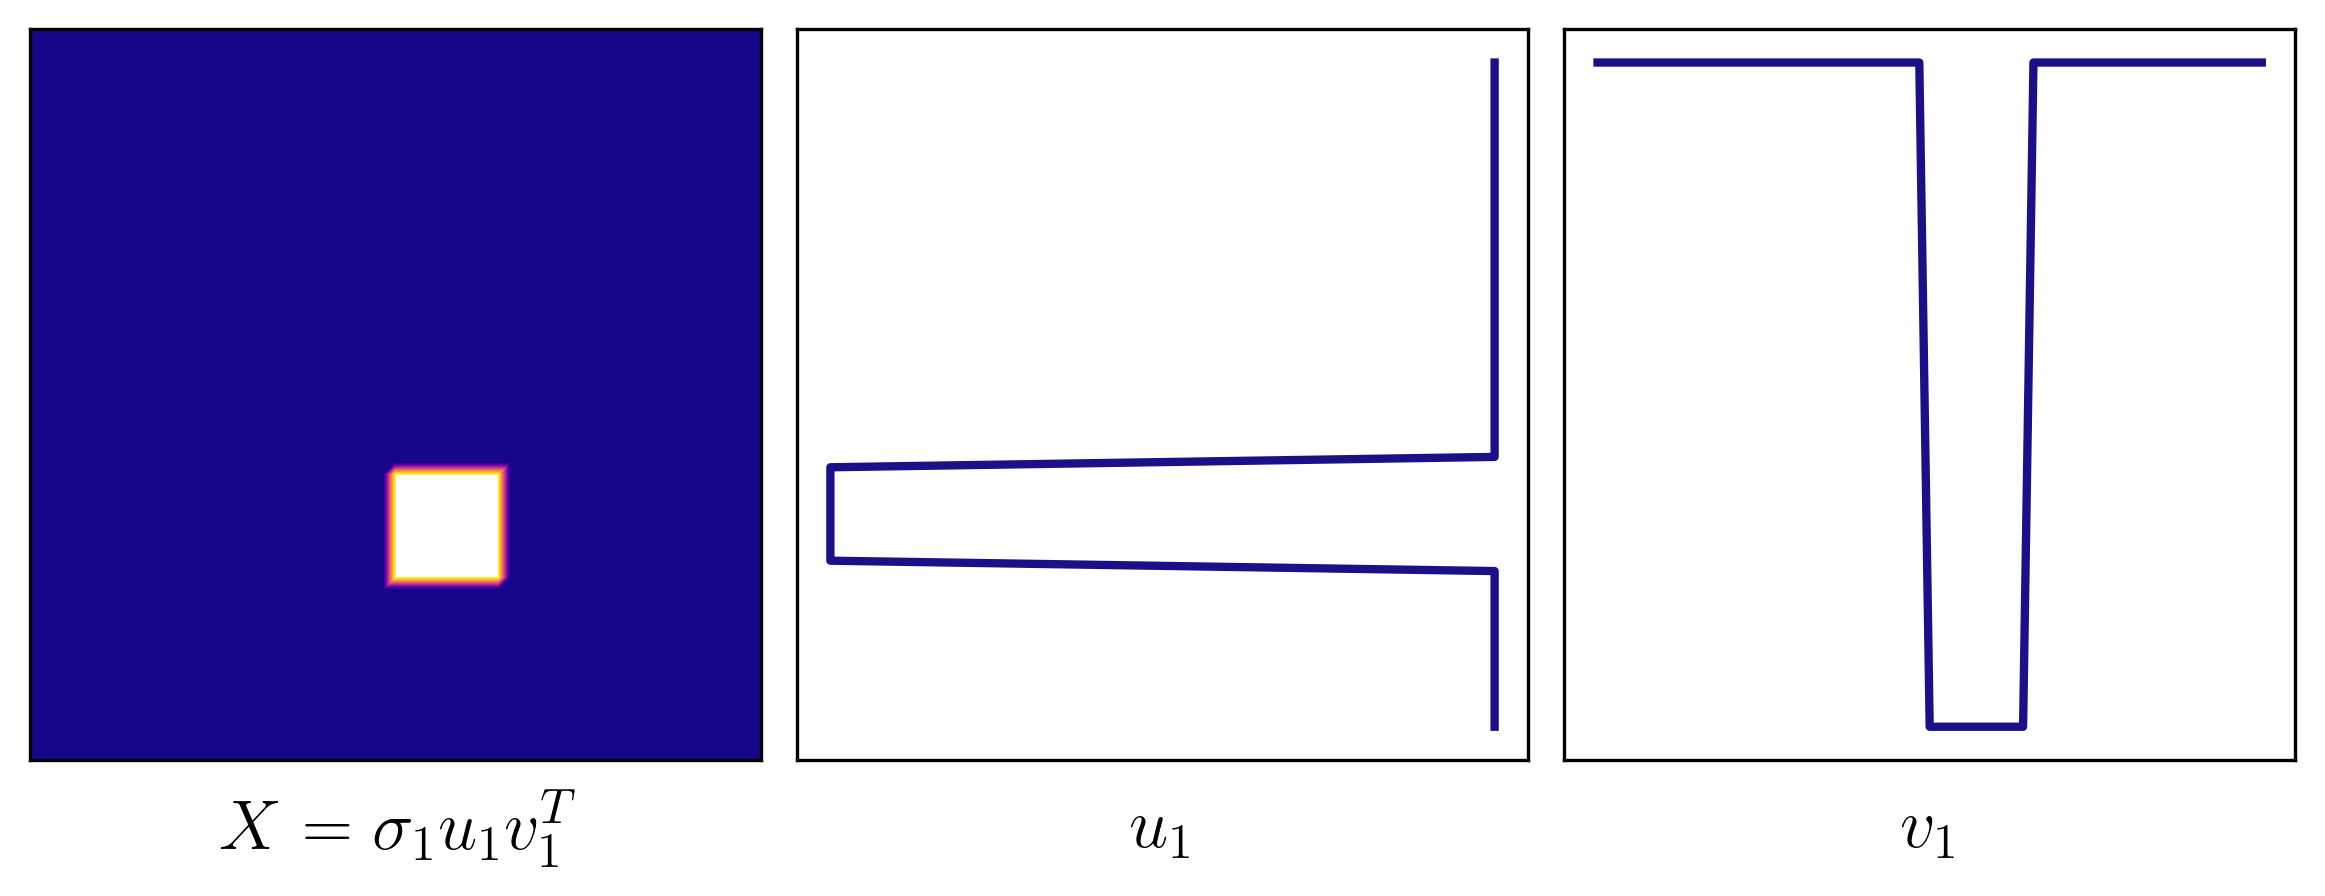
\includegraphics[width=0.6\linewidth]{low_rank_source.png}
\end{center}
$f$ er ofte ``sparse'', og vi kan ofte forvente at $X = \operatorname{mat}(x)$ har $r = \operatorname{rank}(X) \ll N = n^2$:
\begin{itemize}
  \item<2-> $X = \sum_{i=1}^r \sigma_i u_i v_i^T$: $f$ er en sum av ytre-produkter, parametrisert av $u_i,v_i \in \mathbb{R}^n$
  \item<3-> \textbf{Idé:} Let kun etter $X \in \mathcal{M}_r$ hvor $\mathcal{M}_r$ er settet av alle rang-$r$-matriser
\end{itemize}
\end{frame}


\begin{frame}{Lavrang-formuleringen}
Vi definerer kostnadsfunksjonen $\Phi: \mathbb{R}^{n \times n} \to \mathbb{R}$,
\begin{equation*}
  \Phi(X) = \frac{1}{2} \| K x - y \|_{M_\partial}^2
  + \frac{\lambda^2}{2} \| W x \|_M^2
\end{equation*}
\pause
Vi ønsker å minimere $\Phi$ under betingelsen $X \in \mathcal{M}_r$,
\begin{equation*}
  \min_{X \in \mathbb{R}^{n \times n}} \Phi(X)
  \quad \text{s.t.} \quad X \in \mathcal{M}_r
\end{equation*}
\pause
Dynamisk lavrang-tilnærming (DLRA) er en naturlig metode for denne problemstillingen \cite{kochDynamicalLowrankApproximation2007}.
\end{frame}


\begin{frame}{Dynamisk lavrang-tilnærming (DLRA)}
\begin{columns}[T]
  \begin{column}{0.7\textwidth}
    \begin{itemize}
      \item<2-> Søkeretning $D^{(i)}$, steglengde $\alpha_i$
      \item<3-> $X^{(i+1)} = X^{(i)} + \alpha_i \mathcal{P}_{X^{(i)}}(D^{(i)})$
      \item<4-> $\mathcal{P}_{X^{(i)}}(D^{(i)})$ er en projeksjon til planet $\mathcal{T}_{X^{(i)}}(\mathcal{M}_r)$
      \item<5-> \textbf{Men:} DLRA konvergerer sakte for $D^{(i)} = -\nabla \Phi$
      \item<6-> \textbf{Løsning:} $\Phi$ er kvadratisk med SPD Hessian; hva om vi velger $\{D^{(i)}\}$ ved bruk av konjugerte gradienter (CG) i stedet?
    \end{itemize}
  \end{column}
  \begin{column}{0.4\textwidth}
    \centering
    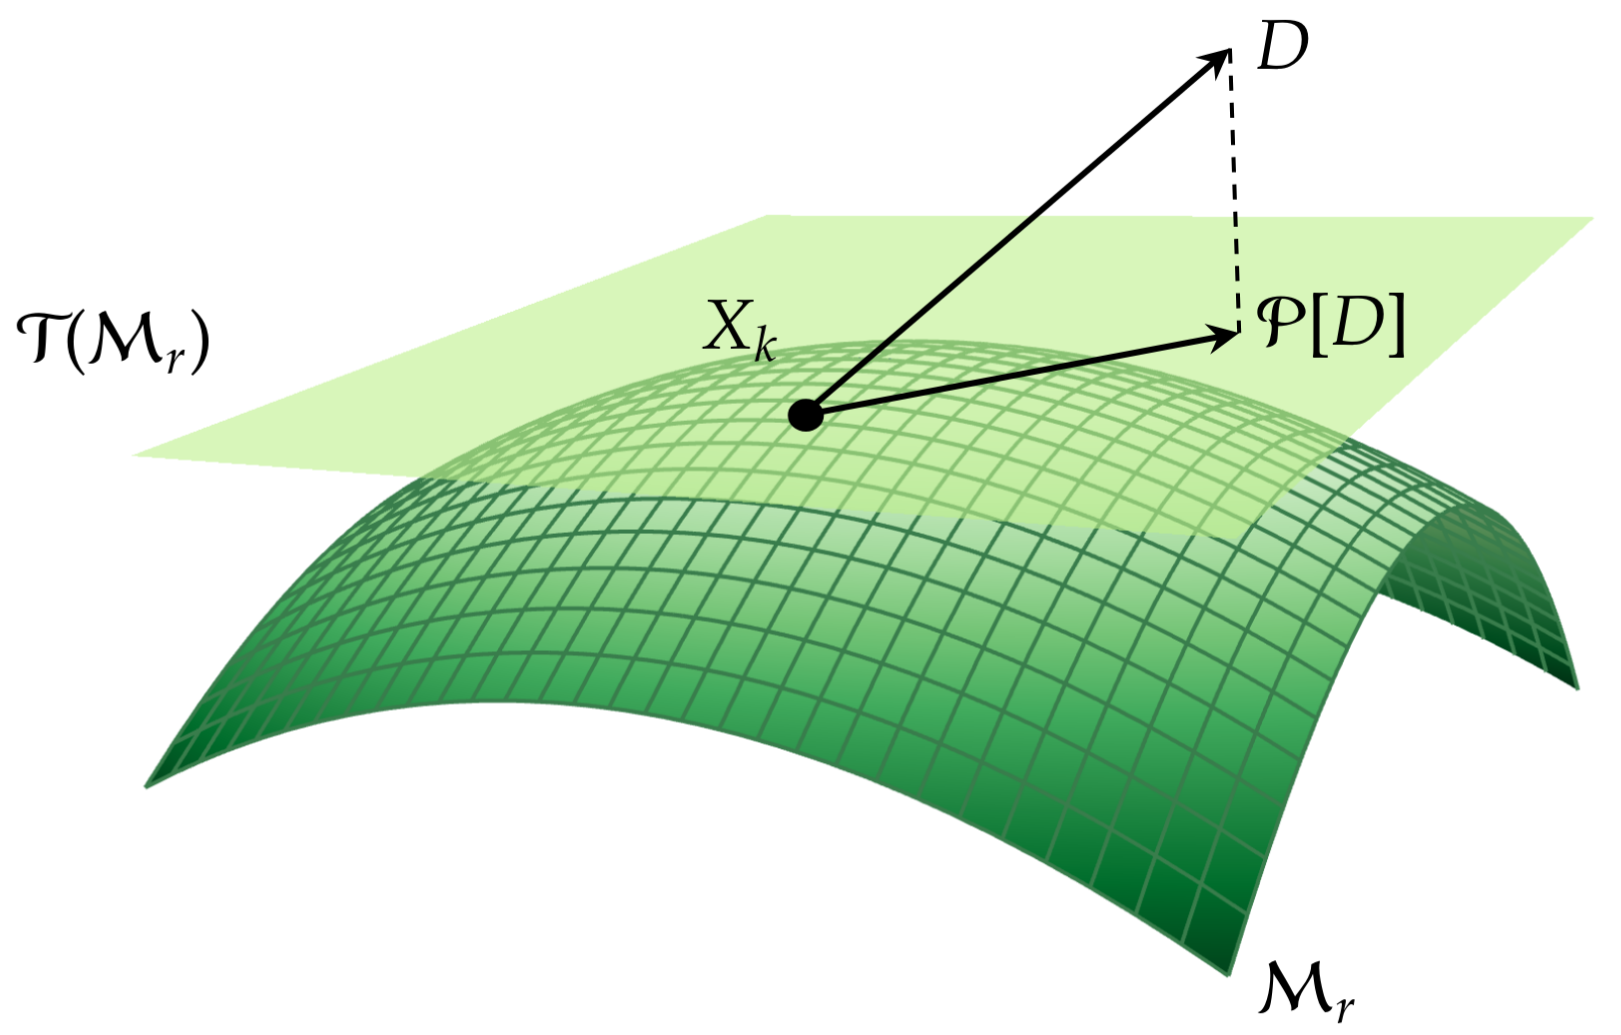
\includegraphics[width=\linewidth]{low_rank_manifold}
  \end{column}
\end{columns}
\end{frame}


\begin{frame}{DLRA med konjugerte gradienter (DLRA-CG)}
Vi bytter ut $D^{(i)} = -\nabla \Phi$ med $\{D^{(i)}\}$ fra CG i DLRA-metoden til Schotthöfer et al \cite{schotthoferLowrankLotteryTickets2022}:

\onslide<2->{
\begin{equation*}
    \alpha_i = \frac{\|G^{(i)}\|_F^2}{\langle D^{(i)},\, H D^{(i)}\rangle_F},
    \quad
    D^{(i+1)} = -G^{(i+1)} + \beta_i D^{(i)},
    \quad
    \beta_i = \frac{\|G^{(i+1)}\|_F^2}{\|G^{(i)}\|_F^2}
\end{equation*}
hvor $G^{(i)} = \nabla \Phi$.
}

\begin{itemize}
  \item<3-> Vi foreslår også en prekondisjonert variant (DLRA-PCG) for å akselerere konvergens
  \item<4-> Restartet CG finner $G^{(i)} = \nabla \Phi$ på nytt hver $N_r$-te iterasjon
\end{itemize}
\end{frame}

% =====================================================================
\section{DLRA-CG: resultater}
% =====================================================================

\begin{frame}{DLRA-CG: antall iterasjoner}
  \centering
  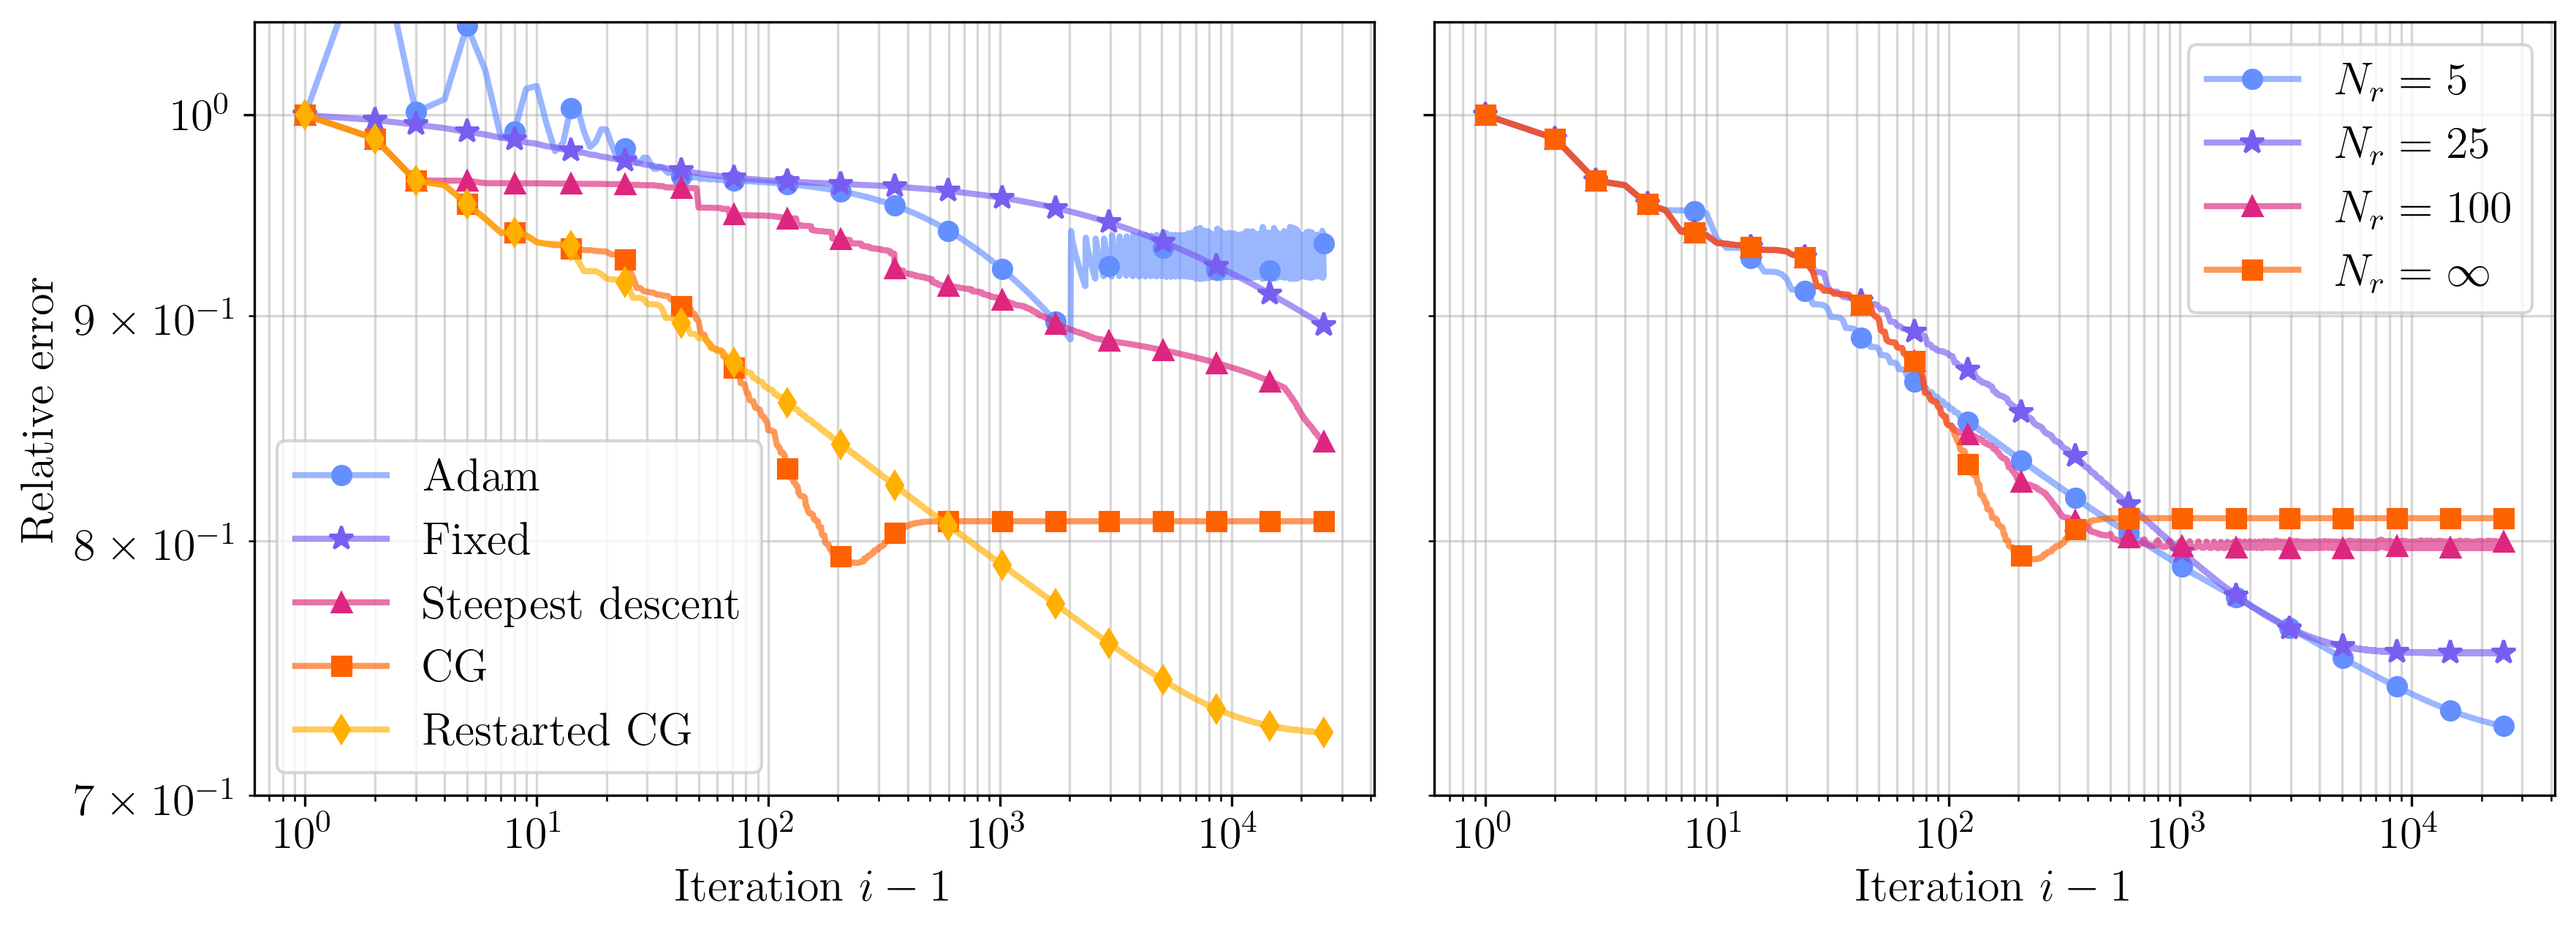
\includegraphics[width=0.8\linewidth]{number_of_iterations.png}
  \par\medskip
  \footnotesize Relativ feil versus antall iterasjoner for DLRA ved bruk av ulike $D^{(i)}$.
\end{frame}


\begin{frame}{DLRA-CG: lavrang-løsninger}
  \centering
  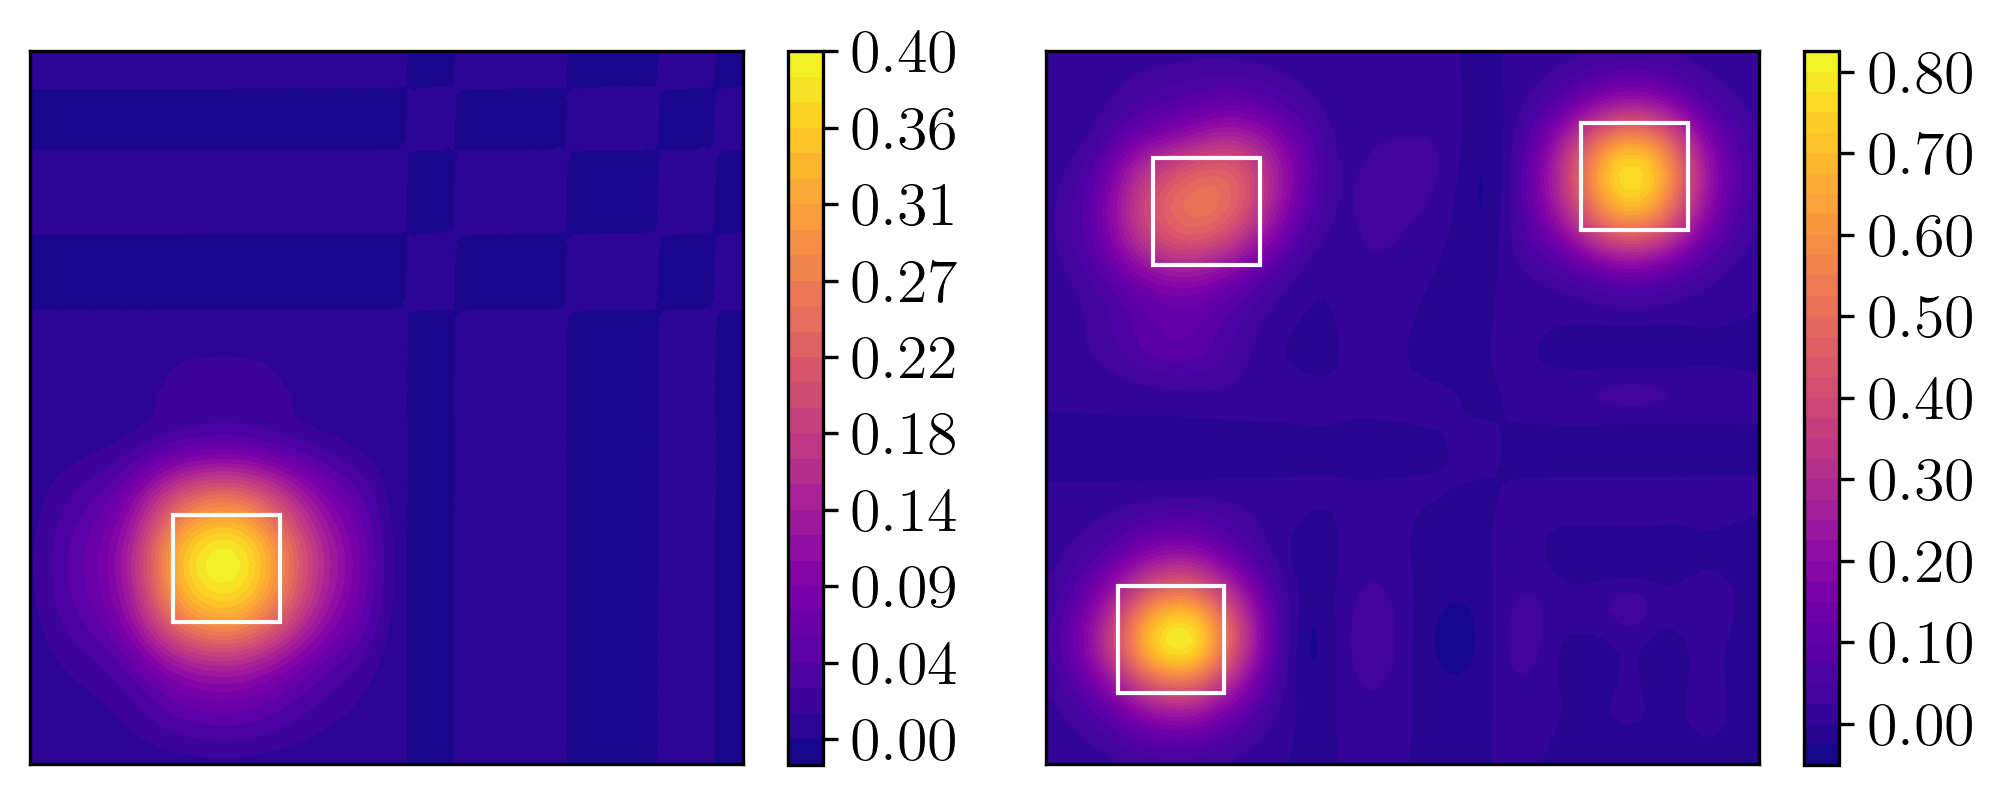
\includegraphics[width=0.8\linewidth]{low_rank_restarted_CG.png}
  \par\medskip
  \footnotesize En rang-1-løsning (venstre) og en rang-2-løsning (høyre). Sanne løsninger markert som hvite kvadrater.
\end{frame}

% =====================================================================
\section{Konklusjon}
% =====================================================================

\begin{frame}{Konklusjon}
  \begin{itemize}
    \item Matrise-fri rSVD løser problemer som tidligere var beregningsmessig uegnet, med liten forskjell i kvaliteten på løsningene
    \item DLRA-CG akselererer konvergens betydelig, og finner lavrang-løsninger med lavere feil enn fullrang-løsninger
  \end{itemize}
  \vspace{1.5em}
  \centering \Large Takk. Spørsmål?
\end{frame}

\appendix

\begin{frame}[allowframebreaks]{Referanser}
  \printbibliography
\end{frame}

% =====================================================================
\section{Appendiks}
% =====================================================================

\begin{frame}{Appendiks i}
\centering
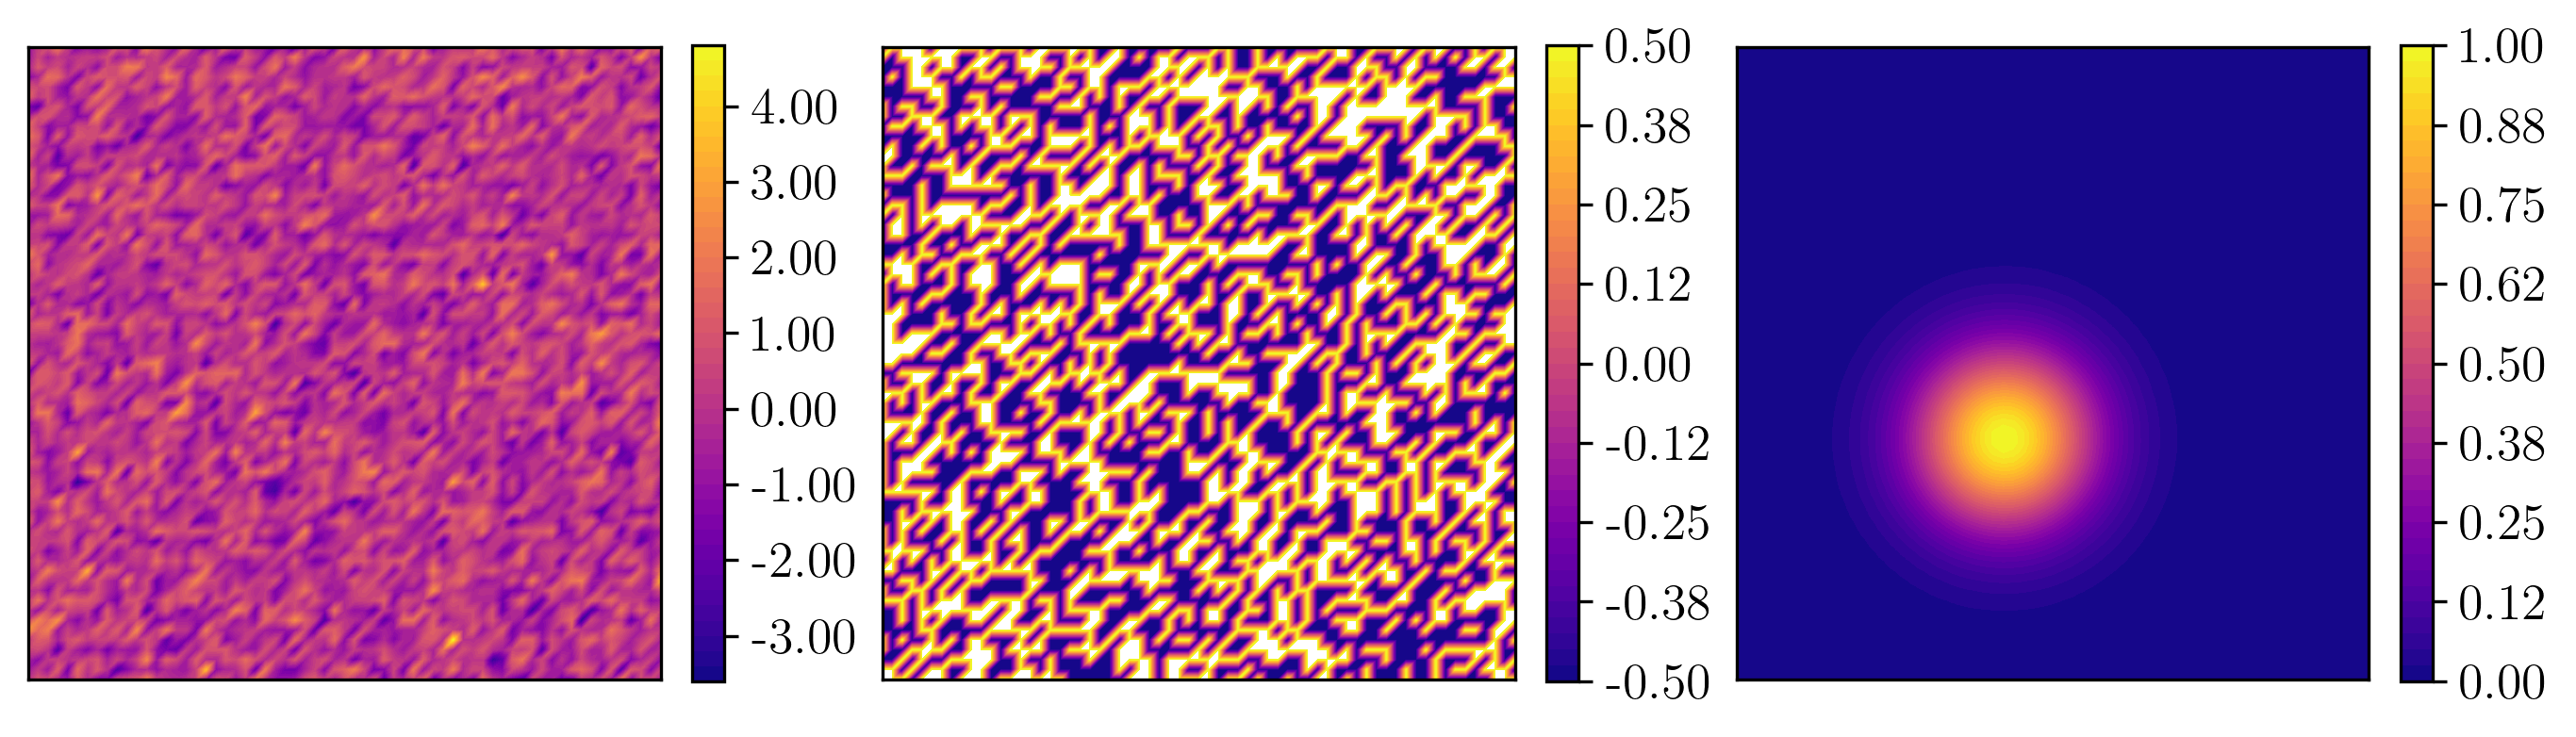
\includegraphics[width=1.0\linewidth]{random_test_vectors.png}
\par\medskip
\footnotesize Valg av fordelingen til $\psi$ i samplingssteget $K \psi$ kan forbedre rang-$k$-tilnærmingen til $K$.
\end{frame}


\begin{frame}{Appendiks ii}
\centering
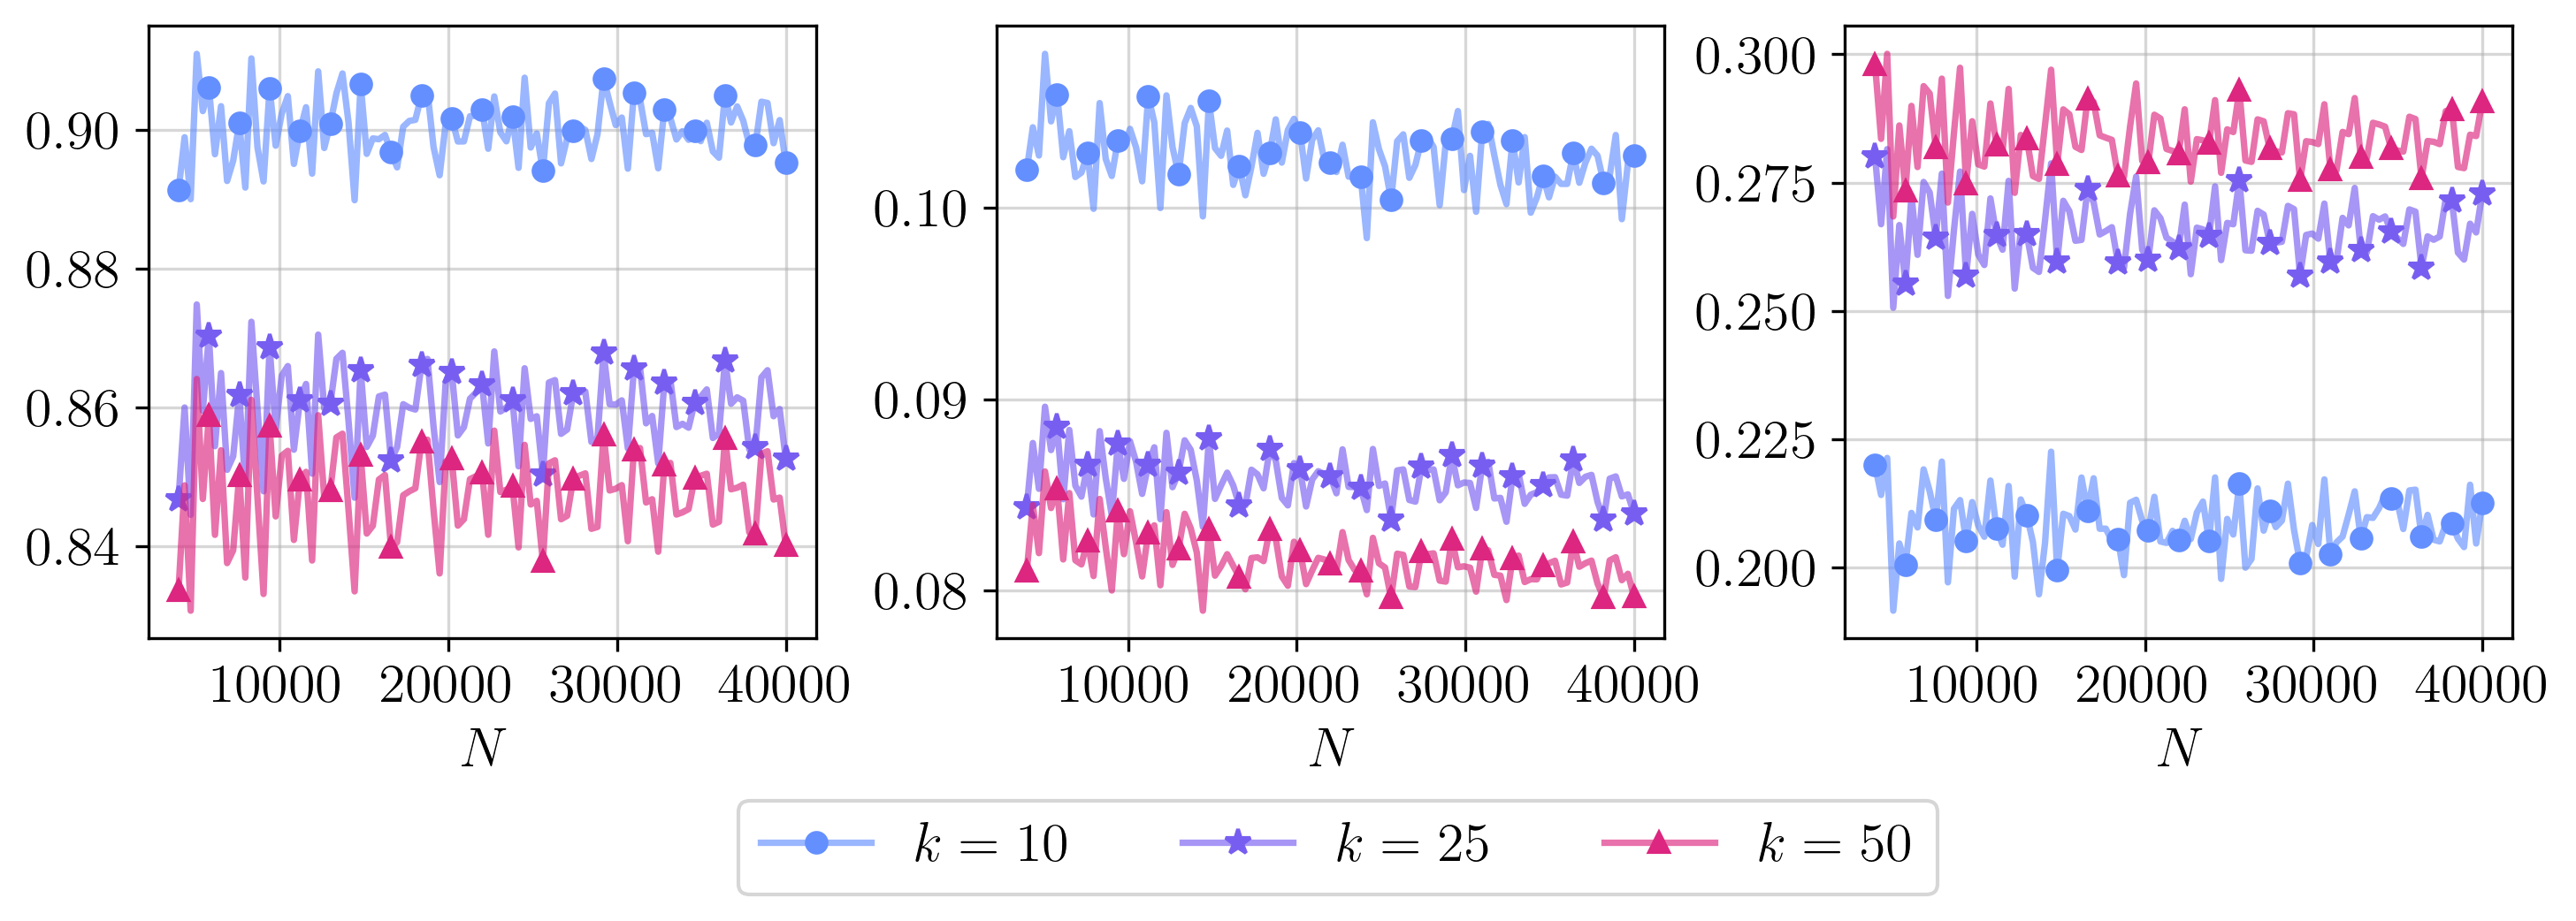
\includegraphics[width=1.0\linewidth]{mesh_resolution_effect.png}
\par\medskip
\footnotesize Oppløsningen $N$ til meshet påvirker ikke valg av $k$.
\end{frame}


\begin{frame}{Appendiks iii}
\centering
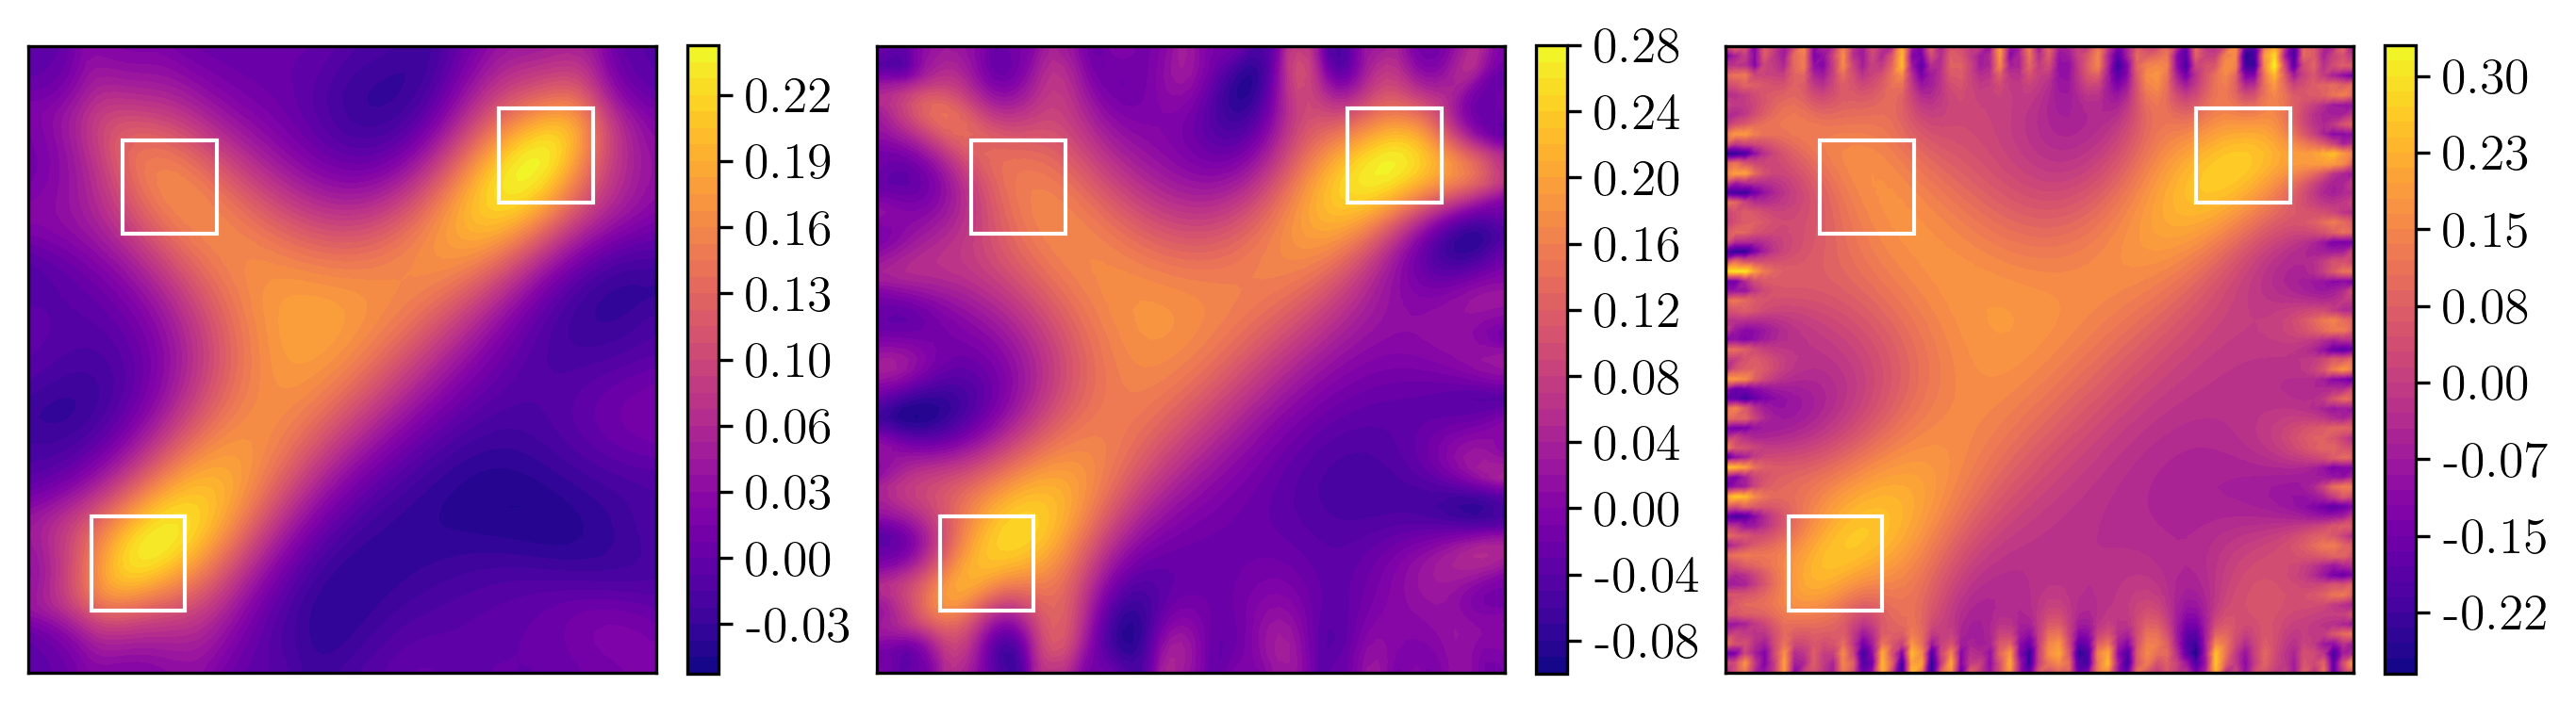
\includegraphics[width=1.0\linewidth]{reconstruction_noisy_problem.png}
\par\medskip
\footnotesize Valg av $k$ fungerer som regularisering for problemer med støy, på samme måte som trunkert SVD. Fra venstre til høyre: $k = 20,\,60,\,150$.
\end{frame}


\begin{frame}{Appendiks iv}
\centering
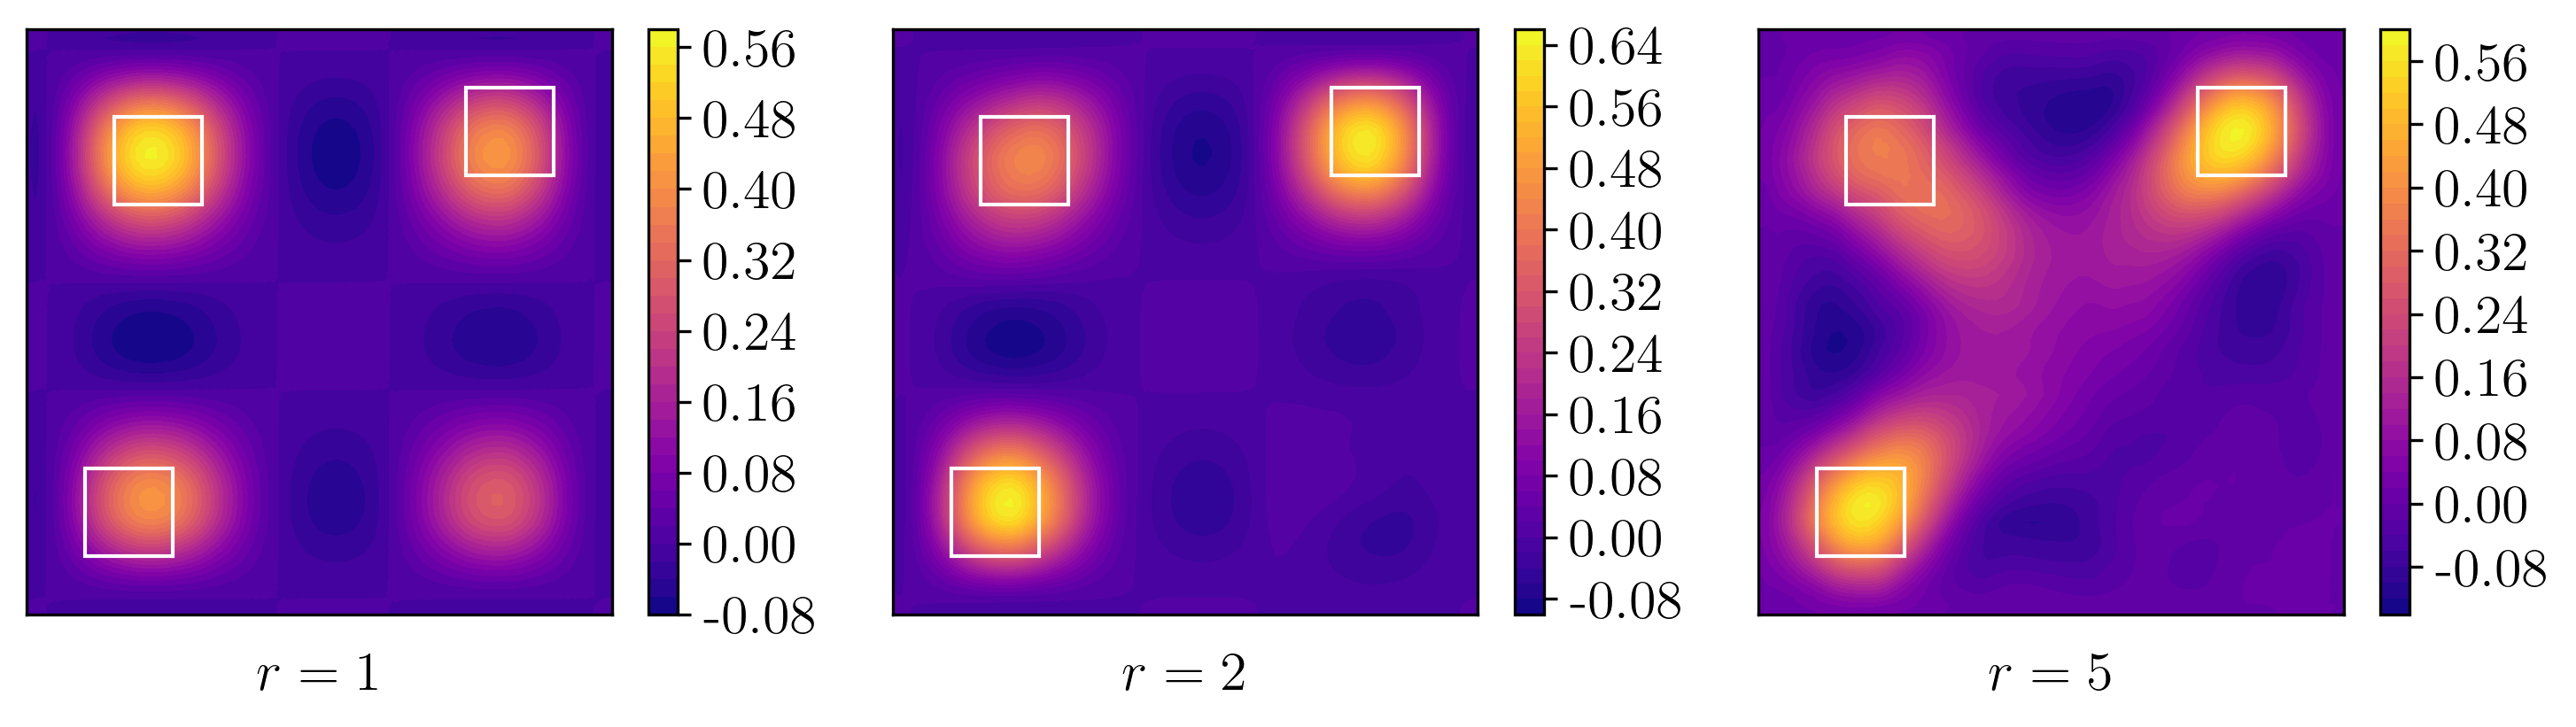
\includegraphics[width=1.0\linewidth]{low_rank_different_r_II.png}
\par\medskip
\footnotesize Feil valg av løsnings-rangen $r$ kan introdusere uønskede kilder.
\end{frame}


\begin{frame}{Appendiks v}
\centering
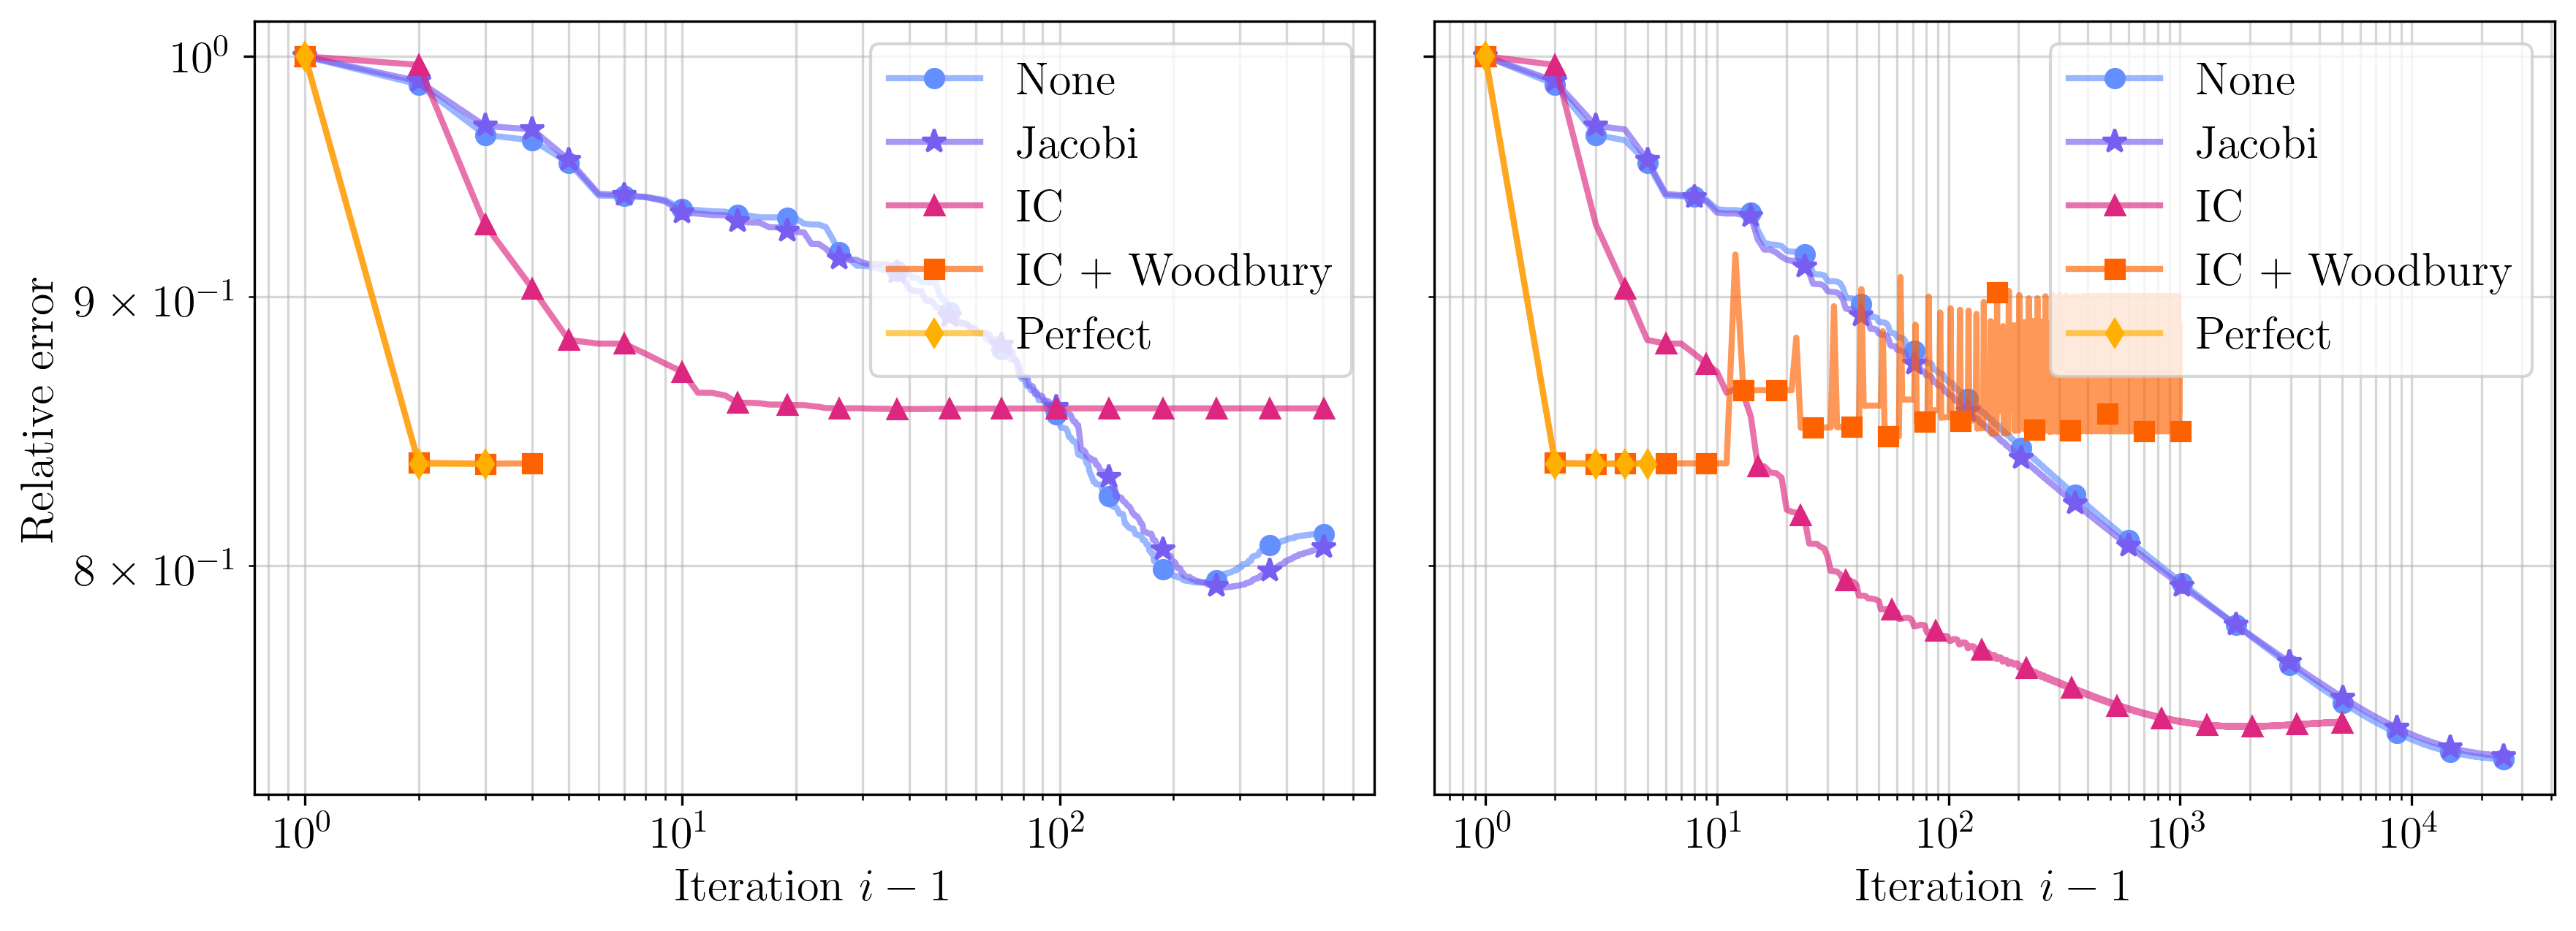
\includegraphics[width=1.0\linewidth]{number_of_iterations_preconditioners.png}
\par\medskip
\footnotesize Prekondisjonert CG akselererer konvergensen ytterligere.
\end{frame}

\end{document}
